\section{Reduction to coupled first order differential equations}

The fundamental problem we wish to solve is to evolve the wave equation on Schwarzschild spacetime with a source. However, to begin to address this problem, I implemented a one dimensional wave equation solver in C++ using the Discontinuous Galerkin method in flat spacetime. The wave equation in flat spacetime is given, in several different forms, by
\begin{eqnarray}
  \Box\psi=0\\
  \frac{\partial^2\psi}{\partial t^2}=\nabla\psi\\
  \frac{\partial^2\psi}{\partial t^2}=\frac{\partial^2 \psi}{\partial r^2}
\end{eqnarray}
where the final form is specialized to one dimension. To numerically integrate this, it is necessary to reduce this second order differential equation to three coupled differential first order differential equations. There is a classical solution to this problem, which we follow. We introduce variables $\rho=\frac{\partial \psi}{\partial t}$ and $\phi = \frac{\partial\psi}{\partial r}$. With these definitions, and remembering that we want time evolution equations rather than spatial evolution equations, the three coupled equations become
\begin{eqnarray}
  \frac{\partial\psi}{\partial t} = \rho\\
  \frac{\partial\rho}{\partial t} = \frac{\partial \phi}{\partial r}\\
  \frac{\partial\phi}{\partial t} = \frac{\partial \rho}{\partial r}
\end{eqnarray}
This system of equations can be rewritten
\begin{equation}
  \frac{\partial u}{\partial t} = A\frac{\partial u}{\partial r} + B\nonumber\\
  \frac{\partial u}{\partial t} = RHS(u,t)
  \label{matrixdiff}
\end{equation}
where $u$ is the state vector consisting of $u=(\psi,\rho,\phi)$, and $A$ and $B$ are matrices. RHS stands for Right Hand Side. The C++ code has been implemented for wave equations of this generalized form, which encompases wave equations on a Schwarzschild spacetime.



\section{Spatial grids}
Our code solves a wave equation, which must first calculate a spatial derivative then integrate in time to solve a differential equation. For the spatial derivative part of the scheme, we make use of the Discontinuous Galerkin method to compute spatial derivatives, as a replacement for a finite difference scheme. Its has three primary benefits. One is that it naturally handles discontinuities in the evolved field, which is important to the effective source approach that we use when calculating orbits with a source in curved spacetime. The second is that its accuracy scales exponentially with increasing polynomial order. The third is that its accuracy scales as a power law with decreasing element size, giving a second strong way to reduce the truncation error.


\subsection{Finite difference schemes}
The classic solution to the spatial derivative problem is the finite difference scheme. In a one dimensional finite difference scheme, space is discretized into points on a line. The spatial derivative is calculated using a stencil of points that is symmetric about the point where one wants to know the spatial derivative, and extends $n-1$ points beyond to either side, where $n$ is the order of the expansion. The spatial derivative is calculated from a weighted sum of the points included in the stencil, where some of the weights are negative. A stencil with $2n-1$ points in it, in one dimension, corresponds to an $n$th order expansion. It is possible to expand any order of derivative to any order of expansion. A first derivative, to second order accuracy, given by:
\begin{equation}
  D_r^{(2)}=\frac{1}{h}(-\frac{1}{2}f_{-1}+\frac{1}{2}f_1)
\end{equation}
Here the $f_{-1}$ and $f_1$ indicate the function evaluated at the grid point to either side of the $0$th grid point, where the derivative is evaluated. Here $h$ is the spacing between grid points. A first derivative, to third order accuracy, is given by:
\begin{equation}
  D_r^{(3)}=\frac{1}{h}(\frac{1}{12}f_{-2}-\frac{2}{3}f_{-1}+\frac{2}{3}f_1-\frac{1}{12}f_2)
\end{equation}
Notice how no first order derivative includes the central point in its stencil. In contrast, a second derivative to second order accuracy is given by:
\begin{equation}
  D_r^{\prime (2)}=\frac{1}{h^2}(f_{-1}-2f_0+f_1)
\end{equation}
This derivative is symmetric, while the first derivative is antisymmetric.

It is possible to extend these stencils to two and three dimensions. When considering parallelization using OpenMP, issues of synchronization must be considered. When parallelizing over many nodes, the spatial grid gets divided into blocks. At the ends of each block, the boundary cells need information from the neighboring cells to calculate the spatial derivative. For an order $n$ derivative, $n-1$ boundary cells are synchronized into buffer zones both to the left and to the right at each time step. In our code, this is not necessary, since we have parallelized with OpenMP, which uses shared memory within one node, across several (16) cores.

\subsection{The Disctontinuous Galerkin method}
The Discontinuous Galerkin method breaks space into segments called elements. Within each element, the value of the field is represented by the sum of $n$ interpolating polynomials of order $n$, where $n$ is the order of the element. There are $n+1$ unevenly spaced nodes in the element, clustered toward the edges. At each node, exactly one of the interpolating polynomials takes on a value of one while the others are zero. An interpolating Lagrange polynomial has a functional form:
\begin{equation}
  \ell_i(r)=\prod_{j=1,j\ne i}^{n}\frac{r-\xi_j}{\xi_i-\xi_j}
\end{equation}
where $\xi_i$ is a location of a node and where $r$ is an arbitrary position~\cite{dghesthaven}. 


Omitting the details of the derivation of this method, which can be found in Reference~\cite{dghesthaven}, the procedure for calculating the spatial derivative in one dimension is to first calculate the Legendre polynomials, rescaled by a factor depending upon their order. $\tilde{P}_n(r)=\frac{P_n(r)}{\sqrt{\gamma_n}}$ where $\gamma_n=\frac{2}{2n+1}$. The following procedure of differentiation and matrix inversion can be used to calculate the derivative matrix for each element, $D_r$~\cite{dghesthaven}.
\begin{equation}
  V_{ij}=\tilde{P}_j(r_i)
\end{equation}
\begin{equation}
  V_{r,(i,j)}=\frac{d\tilde{P}_j}{dr}|_{r_j}
\end{equation}
\begin{equation}
  V^TD_r^T=(V_r)^T
\end{equation}
In practice, we use a custom package, the Template Numerical Toolkit (TNT) library and JAMA, to invert the equation using LU decomposition. Beware! TNT and JAMA are not thread safe, and cannot be used with shared memory parallelization. They result in race conditions, and it was ultimately necessary to rewrite the parallelized portion of the code to avoid the TNT classes.

The Discontinuous Galerkin method helps damp error introduced by discontinuities in the field, provided they remain at element boundaries. We make use of this in our self-force calculations in the neighborhood of the particle, to be described in Chapter~\ref{ellipticalorb}. The numerical flux is a way of accounting for the discontinuity in the flow between neighboring elements. There are multiple ways of calculating this flux, but in our code, we use a version relevant to linear hyperbolic problems, such as Equation~\ref{matrixdiff}, which, recall, is specialized to a one-dimensional problem. In this case, $A=S\Lambda S^{-1}$, for some transformation matrix $S$, where $\Lambda$ is a diagonal matrix. Let $\Lambda^+$ and $\Lambda^-$ be the positive and negative eigenvalues of $\Lambda$, respectively, corresponding to the outgoing and ingoing waves. Then the numerical upwind flux is given by
\begin{equation}
  (\hat{n}\dot F)=S(\Lambda^+ S^{-1} u^- + \Lambda^- S^{-1} u^+)
\end{equation}
This flux, based upon the state vector interior to ($u^-$) and exterior to ($u^+$) the element, at each end of the element, is distributed across the whole element from end to end via the lift matrix~\cite{dghesthaven}.


\section{Time evolution}

Time evolution in our code is handled by a fourth order low storage Runga Kutta method. Instead of the standard fourth order Runga Kutta method, this method takes five sub-timesteps, but only the most recent sub-timestep needs to be stored.

\begin{eqnarray}
  p^{(0)}=u^n
  k^{(i)}=a_ik^{(i-1)}+\delta t RHS(p^{(i-1)},t^n+c_i\delta t)
  p^{(i)}=p^{(i-1)}+b_iK^{(i)}
  u_h^{n+1}=p^{(5)}
\end{eqnarray}
Here steps two and three are repeated for $i=1-5$, first $k$, then $p$, then increase $i$ and repeat. The coefficients $a_i$, $b_i$, and $c_i$ are given in Refence~\cite{dghesthaven}.

\section{Wave equation on flat spacetime}

Using gaussian initial conditions in $\psi$ and setting the $\rho$ initial conditions to the derivative of that gaussian, I have produced the evolution shown in Figure~\ref{gaussWave}. The gausian marches to the right over a number of time steps, hits the periodic boundary conditions, and re-enters the one-dimensional space on the left, eventually returning to its original position. A similar progression can be seen in Figure~\ref{sineWave} for sinusoidal initial conditions.

\begin{figure}
  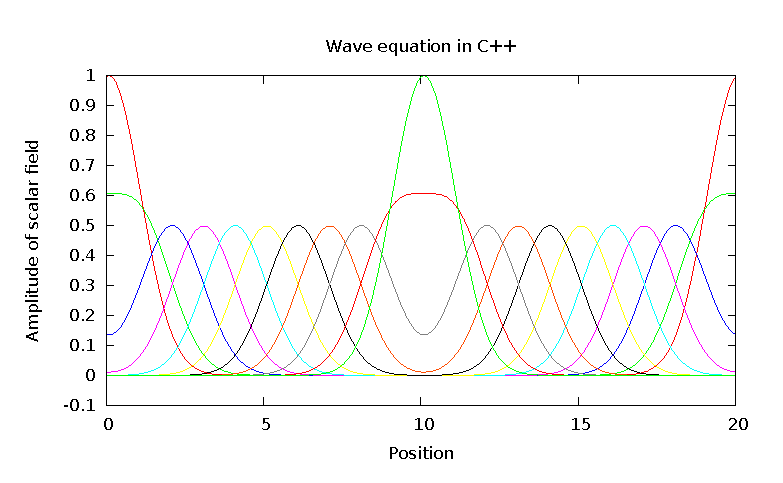
\includegraphics{gaussWave}
  \caption{Waves evolving over time for gaussian initial conditions}
  \label{gaussWave}
\end{figure}

\begin{figure}
  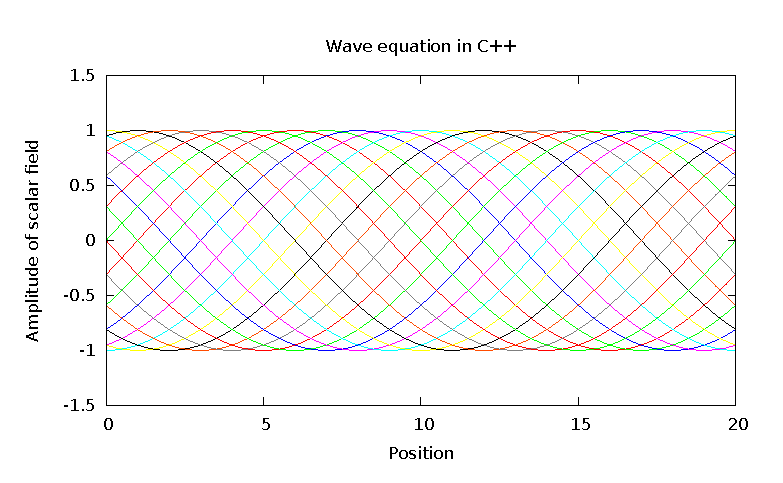
\includegraphics{sineWave}
  \caption{Waves evolving over time for sinusoidal initial conditions}
  \label{sineWave}
\end{figure}

The Discontinuous Galerkin method has truncation error that scales as $h^{n+1}$, where $h$ is the element size and $n$ is the polynomial order of the elements. The $L_2$ error is definied as the square root of the sum of the squared differences across all space, after one complete cycle of the system. The scaling of the $L_2$ error with DG order and with element size is shown in Figures~\ref{scalingorder} and~\ref{scalingelement}. The scaling matches expectations until roundoff error is hit, where the error stops improving with order or smaller element size. Not shown, this same partern was seen for the $L_0$ error, which is the maximum error over all space.

\begin{figure}
  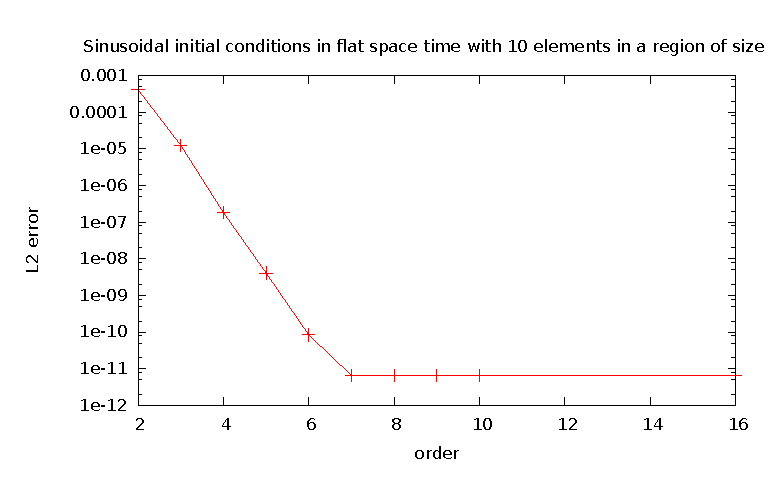
\includegraphics{sinL2WTorder}
  \caption{$L_2$ error scaling with DG order for sinusoidal initial conditions}
  \label{scalingorder}
\end{figure}

\begin{figure}
  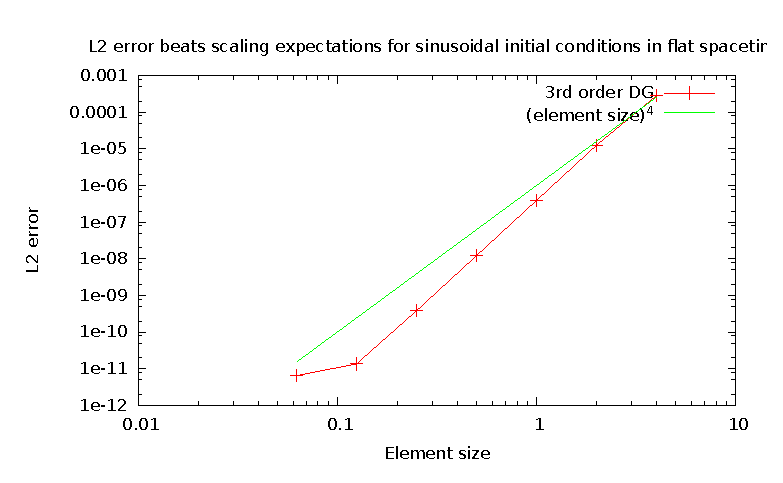
\includegraphics{sinL2WTelement}
  \caption{$L_2$ error scaling with element size for sinusoidal initial conditions}
  \label{scalingelement}
\end{figure}


